\documentclass[10pt]{beamer}

\usetheme[progressbar=frametitle]{metropolis}

\usepackage{appendixnumberbeamer}

\usepackage{booktabs}
\usepackage{blkarray}
%\usepackage{ccicons}
\usepackage{graphicx}
\usepackage{color}

\definecolor{UniBlue}{RGB}{7,82,154}
\definecolor{UniYellow}{RGB}{234,185,12}

%\setbeamercolor{title}{fg=UniBlue, bg = UniYellow}
%\setbeamercolor{frametitle}{fg=UniBlue, bg= UniYellow}
%\setbeamercolor{structure}{fg=UniBlue, bg= UniYellow}
%\setbeamercolor{progress bar}{fg=UniBlue, bg= UniYellow}
\usepackage{xspace}

\title{Simultaneous statistical inference for epidemic trends: the case of COVID-19}
\date{01/10/2020}
\author{Marina Khismatullina \and Michael Vogt}
\setbeamertemplate{frame footer}{Simultaneous statistical inference for epidemic trends: the case of COVID-19}
\metroset{block=fill}
% \titlegraphic{\hfill\includegraphics[height=1.5cm]{logo.pdf}}

\newcommand{\Prob}{\mathrm{P}}
\newcommand{\E}{\mathbb{E}}
\newcommand{\Var}{\mathrm{Var}}
\newcommand{\Cov}{\mathrm{Cov}}
\newcommand{\Corr}{\mathrm{Corr}}
\newcommand{\sgn}{\text{sgn}}
\newtheorem{prop}{Proposition}
\newcommand{\ind}{\boldsymbol{1}\Big( \frac{t}{T} \in \mathcal{I}_k \Big)} % indicator function
\newcommand{\indsmall}{\boldsymbol{1}\big( \frac{t}{T} \in \mathcal{I}_k \big)} % indicator function

\begin{document}

\maketitle

\begin{frame}{Table of contents}
  \setbeamertemplate{section in toc}[sections numbered]
  \tableofcontents[hideallsubsections]
\end{frame}

\section{Introduction}


\begin{frame}{Motivation}
	\textbf{Research question:}	
	How do outbreak patterns of COVID-19 compare across countries?
	\begin{figure}
    		\centering
    		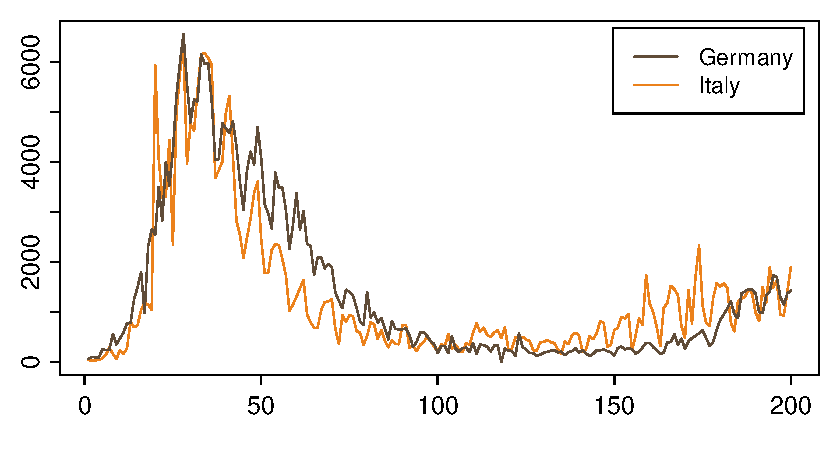
\includegraphics[height=0.45\textheight]{plots/Germany_and_Italy.pdf}
    		%\caption{Observed new cases per day in Germany and Italy}
    		\label{fig:DEUvsITA}
  	\end{figure}\pause
	\vspace{-3mm}
	\begin{block}{Aim of the paper}
	To develop new inference methods that allow to \textit{identify} and \textit{locate} differences between epidemic time trends.
	\end{block}
\end{frame}

\begin{frame}{Literature}
	Comparison of deterministic trends:
	\begin{itemize}
		\item Park et al. (2009), Degras et al. (2012), Zhang et al. (2012), Hidalgo and Lee (2014), Chen and Wu (2019).
	\end{itemize}\pause
	Studies of COVID-19:
	\begin{itemize}
		\item SIR models: Yang et al. (2020), Wu et al. (2020), De Brouwer et al. (2020).
		\item Time series analysis: Gu et al. (2020), Li and Linton (2020).
	\end{itemize}
\end{frame}


\section{Model}
\begin{frame}{Motivation for the model}
We observe $n$ time series $\mathcal{X}_i = \{X_{it}: 1 \le t \le T \}$ of length $T$.\pause

$X_{it}$ are non-negative integers $\Rightarrow$ can be modelled by a Poisson distribution with time-varying parameter $\lambda_i(t/T)$: $X_{it} \sim P_{\lambda_i(t/T)}$.\pause

Since $\lambda_i(t/T) = \E[X_{it}] = \Var(X_{it})$, we can rewrite $X_{it}$ as
\vspace{-2mm}
\begin{equation*}
X_{it} = \lambda_i\Big(\frac{t}{T}\Big) + u_{it} \quad \text{with} \quad u_{it} = \sqrt{\lambda_i\Big(\frac{t}{T}\Big)} \eta_{it}
\end{equation*}\pause
In applications the variance can be larger than the mean $\Rightarrow$ quasi-Poisson models.
\end{frame}

\begin{frame}{Model}
Quasi-Poisson model:
\begin{equation*}
X_{it} = \lambda_i \Big( \frac{t}{T} \Big) + \sigma\sqrt{\lambda_i \Big( \frac{t}{T} \Big)} \eta_{it},
\end{equation*}\pause
\vspace{-3mm}
where
\begin{itemize}
\item $\lambda_i$ are unknown trend functions on $[0,1]$;\pause
\item $\sigma$ is the overdispersion parameter;\pause
\item $\eta_{it}$ are error terms that are independent across $i$ and $t$ and have zero mean and unit variance.
\end{itemize}
\end{frame}

\section{Testing}
\begin{frame}{Testing problem}

Let $\mathcal{F} :=\{ \mathcal{I}_k \subseteq [0, 1]: 1 \le k \le K\}$ be a family of rescaled time intervals on $[0, 1]$, and let $H_0^{(ijk)}$ be the hypothesis that the functions $\lambda_i$ and $\lambda_j$ are equal on an interval $\mathcal{I}_k$, \pause i.e.
\begin{align*}
H_0^{(ijk)}:\quad  \lambda_i(w) = \lambda_j(w) \text{ for all } w\in \mathcal{I}_k
\end{align*}\pause
We want to test $H_0^{(ijk)}$ simultaneously for all pairs of countries $i$ and $j$ and all intervals $\mathcal{I}_k$ in the family $\mathcal{F}$ and we want to control the familywise error rate (FWER) at level $\alpha$.\pause

Let $\mathcal{M}_0$ be the set of triplets $(i, j, k)$ for which $H_0^{(ijk)}$ holds true. Then, FWER is
\begin{align*}
\text{FWER}(\alpha) = \Prob \Big( \exists (i,j,k) \in \mathcal{M}_0: \text{we reject } H_0^{(ijk)} \Big)
\end{align*}
\end{frame} 


\begin{frame}[label = frame_teststatistic]{Test statistic}
For the given interval $\mathcal{I}_k$ and a pair of time series $i$ and $j$ we calculate
\begin{equation*}
\hat{s}_{ijk,T} = \frac{1}{T h_k} \sum\limits_{t=1}^T \ind (X_{it} -X_{jt}), 
\end{equation*}
%\vspace{-3mm}
where $h_k$ is the length of $\mathcal{I}_k$. \pause $\hat{s}_{ijk,T}$ estimates the average distance between $\lambda_i$ and $\lambda_j$ on $\mathcal{I}_k$. \pause Under certain assumptions, 
\begin{align*}
\Var(\hat{s}_{ijk,T})  & = \frac{\sigma^2}{T^2 h_k^2} \sum\limits_{t=1}^T \ind \Big\{ \lambda_i\Big(\frac{t}{T}\Big) + \lambda_j\Big(\frac{t}{T}\Big) \Big\}
\end{align*}\pause
In order to normalize the variance of the statistic $\hat{s}_{ijk,T}$, we scale it by an estimator of its variance:
\[ \widehat{\Var(\hat{s}_{ijk,T})} = \frac{\hat{\sigma}^2}{T^2 h_k^2} \sum\limits_{t=1}^T \ind (X_{it} + X_{jt} ), \]
with $\hat{\sigma}^2$ being an appropriate estimator of $\sigma^2$. \hyperlink{frame_sigma}{\beamerbutton{Details}}
\end{frame}


\begin{frame}{Test statistic, part 2}
Test statistic for the hypothesis $H_0^{(ijk)}$ is defined as
\begin{equation*}
\widehat{\psi}_{ijk, T} = \frac{\sum\nolimits_{t=1}^T \indsmall (X_{it} -X_{jt})}{\hat{\sigma} \big\{ \sum\nolimits_{t=1}^T \indsmall  (X_{it} + X_{jt} )\big\}^{1/2}}
\end{equation*} \pause
Under certain conditions and under the null, $\widehat{\psi}_{ijk, T}$ can be approximated by a Gaussian version of the test statistic:
\begin{align*}
\phi_{ijk,T} = \frac{1}{\sqrt{2 T h_k}} \sum\limits_{t=1}^T \ind (Z_{it} - Z_{jt}), 
\end{align*}
where $Z_{it}$ are independent standard normal random variables.
\end{frame}

\begin{frame}{Critical values}
How to construct critical values $c_{ijk,T}(\alpha)$?\pause
\begin{itemize} 
\item Traditional approach: $c_{ijk,T}(\alpha) = c_T(\alpha)$ for all $(i,j,k)$. \pause
\item More modern approach: $c_{ijk,T}(\alpha)$ depend on the length $h_k$ of the time interval (D{\"u}mbgen and Spokoiny (2001)).
\end{itemize}\pause
In our context: 
\vspace{-2mm}
\[c_{ijk,T}(\alpha) = c_T(\alpha,h_k) := b_k + q_T(\alpha)/a_k,\] where $a_k = \{\log(e/h_k)\}^{1/2} / \log \log(e^e / h_k)$ and $b_k = \sqrt{2 \log(1/h_k)}$ are scale-dependent constants and $q_T(\alpha)$ is chosen such that we control FWER.
\end{frame}


\begin{frame}{Critical values, part 2}
We want to control FWER:
\begin{align*}
\text{FWER}(\alpha) &= \Prob \Big( \exists (i,j,k) \in\mathcal{M}_0: |\widehat{\psi}_{ijk, T} | > c_{ijk, T}(\alpha) \Big) \\
&= 1 - \Prob \Big( \forall (i,j,k) \in\mathcal{M}_0: |\widehat{\psi}_{ijk, T} | \le c_{ijk, T}(\alpha) \Big)\\
 & =  1 - \Prob \Big( \forall (i,j,k) \in \mathcal{M}_0: a_k \big(|\hat{\psi}_{ijk,T}| - b_k\big) \le q_T(\alpha) \Big)\\
 & = 1 - \Prob\Big( \max_{(i,j,k) \in \mathcal{M}_0} a_k \big( |\hat{\psi}_{ijk,T}| - b_k \big) \le q_T(\alpha) \Big)\\
 & \le \alpha
\end{align*}\pause
Hence, we choose $q_T(\alpha)$ as the $(1-\alpha)$-quantile of the statistic 
\[ \hat{\Psi}_T = \max_{(i,j,k)} a_k \big( |\hat{\psi}_{ijk,T}^0| - b_k \big), \]
where $\hat{\psi}_{ijk,T}^0$ is equal to $\hat{\psi}_{ijk,T}$ under the null.
\end{frame}

\begin{frame}[label = frame_test]{Test procedure}

\begin{enumerate}
	\item Consider the Gaussian test statistic 
	\vspace{-2mm} \[ \Phi_T = \max_{(i,j,k)} a_k \big( |\phi_{ijk,T}| - b_k \big), \] where $a_k$ and $b_k$ are scale-dependent constants and $\phi_{ijk, T}$ are weighted averages of the differences of standard normal random variables.\pause
	\item Compute a $(1-\alpha)$-quantile $q_{T, \text{Gauss}} (\alpha)$ of $\Phi_T$ by Monte Carlo simulations.\pause
	\item Adjust $q_{T, \text{Gauss}} (\alpha)$ by the scale-dependent constants \vspace{-2mm}  \[c_{T,\text{Gauss}}(\alpha,h_k) = b_k + q_{T,\text{Gauss}}(\alpha)/a_k\] \pause
\end{enumerate}
\vspace{-5mm}
\begin{block}{Test procedure}
For the given significance level $\alpha \in (0,1)$ and for each $(i,j,k)$, reject $H_0^{(ijk)}$ if $|\widehat{\psi}_{ijk,T}| > c_{T,\text{Gauss}}(\alpha,h_k)$.

\end{block}
\end{frame}

\section{Theoretical properties}
\begin{frame}{Assumptions}
\begin{itemize}
\onslide<1->\item[$\mathcal{C}1$] \label{C1} The functions $\lambda_i$ are uniformly Lipschitz continuous: $|\lambda_i(u) - \lambda_i(v)| \le L |u-v|$ for all $u, v \in [0,1]$.
\onslide<2->\item[$\mathcal{C}2$] \label{C2} $0 < \lambda_{\min} \le \lambda_i(w) \le \lambda_{\max} < \infty$ for all $w \in [0, 1]$ and all $i$. 
\onslide<3->\item[$\mathcal{C}3$] \label{C3} $\eta_{it}$ are independent both across $i$ and $t$.
\onslide<4->\item[$\mathcal{C}4$] \label{C4} $\E[\eta_{it}] = 0$, $\E[\eta_{it}^2] = 1$ and $\E[|\eta_{it}|^\theta] \le C_\theta < \infty$ for some $\theta > 4$. 
\onslide<5->\item[$\mathcal{C}5$] \label{C5} $h_{\max} = o(1/\log T)$ and $h_{\min} \ge CT^{-b}$ for some $b \in (0,1)$.
\onslide<6>\item[$\mathcal{C}6$] \label{C6} $p := \{ \# (i, j, k) \} = O(T^{(\theta/2)(1-b)-(1+\delta)})$ for some small $\delta > 0$.
\end{itemize}
\end{frame}


\begin{frame}{Theoretical properties}
\begin{prop}\label{prop1}
Let $\mathcal{M}_0$ be the set of triplets $(i, j, k)$ for which $H_0^{(ijk)}$ holds true. Then under $\mathcal{C}1 - \mathcal{C}6$, it holds that 
\vspace{-2mm}
\begin{align*}
 \Prob\Big( \forall (i,j,k) \in \mathcal{M}_0: |\hat{\psi}_{ijk,T}| \le c_{T,\textnormal{Gauss}}(\alpha,h_k) \Big) \ge 1 - \alpha + o(1)
\end{align*}
\end{prop}\pause
\begin{prop}\label{prop2}
Consider a sequence of functions $\lambda_{i} = \lambda_{i,T}$, $\lambda_{j} = \lambda_{j, T}$ such that 
\begin{equation}\label{eq:localt}
\exists \, \mathcal{I}_{k}:  \lambda_{i, T}(w) - \lambda_{j, T}(w) \ge c_T \sqrt{\log T / (T h_{k})} \,\, \forall w \in \mathcal{I}_{k},
\end{equation} and $c_T \rightarrow \infty$ faster than $\frac{\sqrt{\log T}\sqrt{\log \log T}}{\log \log \log T}$. \pause Let $\mathcal{M}_1$ be the set of triplets $(i, j, k)$ for which \eqref{eq:localt} holds true. Then under $\mathcal{C}1 - \mathcal{C}6$, it holds that
\vspace{-2mm}
\begin{equation*}
\Prob\Big( \forall (i,j,k) \in \mathcal{M}_1: |\hat{\psi}_{ijk,T}| > c_{T,\textnormal{Gauss}}(\alpha,h_k) \Big) = 1 - o(1)
\end{equation*}
\end{prop}
\end{frame}

\section{Application}

\begin{frame}{Graphical representation}
How to represent the results of the test? Plot the results of pairwise comparison $\mathcal{F}_{\text{reject}}(i, j)$.\pause
\begin{block}{Minimal intervals}
An interval $\mathcal{I}_k \in \mathcal{F}_{\text{reject}}(i, j)$ is called \textbf{minimal} if there is no other interval $\mathcal{I}_{k^\prime} \in \mathcal{F}_{\text{reject}}(i, j)$ with $\mathcal{I}_{k^\prime} \subset \mathcal{I}_k$. The set of minimal intervals is denoted $\mathcal{F}_{\text{reject}}^{\min} (i, j)$.
\end{block}\pause
We can make very similar confidence statement about the set of minimal intervals as well:
\begin{align*}
 \Prob\Big( \forall (i,j,k) \in \mathcal{M}_0: \mathcal{I}_k \notin \mathcal{F}_{\text{reject}}^{\min} (i, j) \Big) \ge 1 - \alpha + o(1)
\end{align*}
\end{frame}

\begin{frame}{Application setting}
\begin{itemize}
\item Five countries: Germany, Italy, Spain, France and UK; $T = 120$. \pause
\item $\alpha = 0.05$.\pause
\item Lengths of the time intervals $7, 14, 21, 28$ days. The intervals start at days $1, 8, 15, \ldots$ and $4, 11, 19, \ldots$ \pause
\vspace{-2mm}
\end{itemize}
	\begin{figure}
		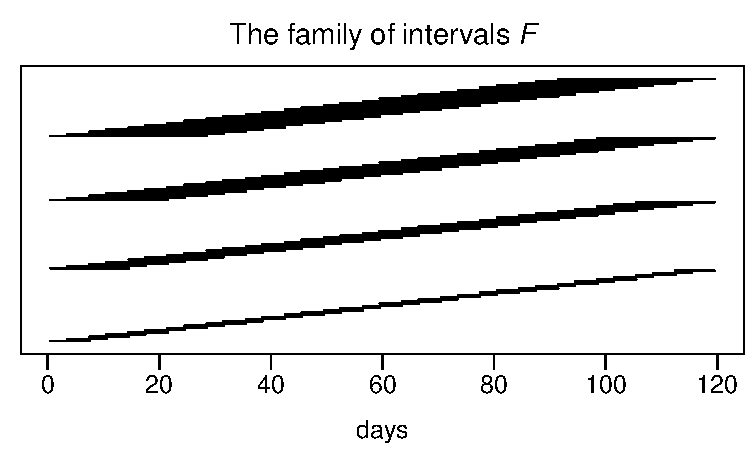
\includegraphics[width = 0.85\textwidth]{plots/all_intervals}
	\end{figure}
\end{frame}

\begin{frame}{Application results}
	\begin{figure}
		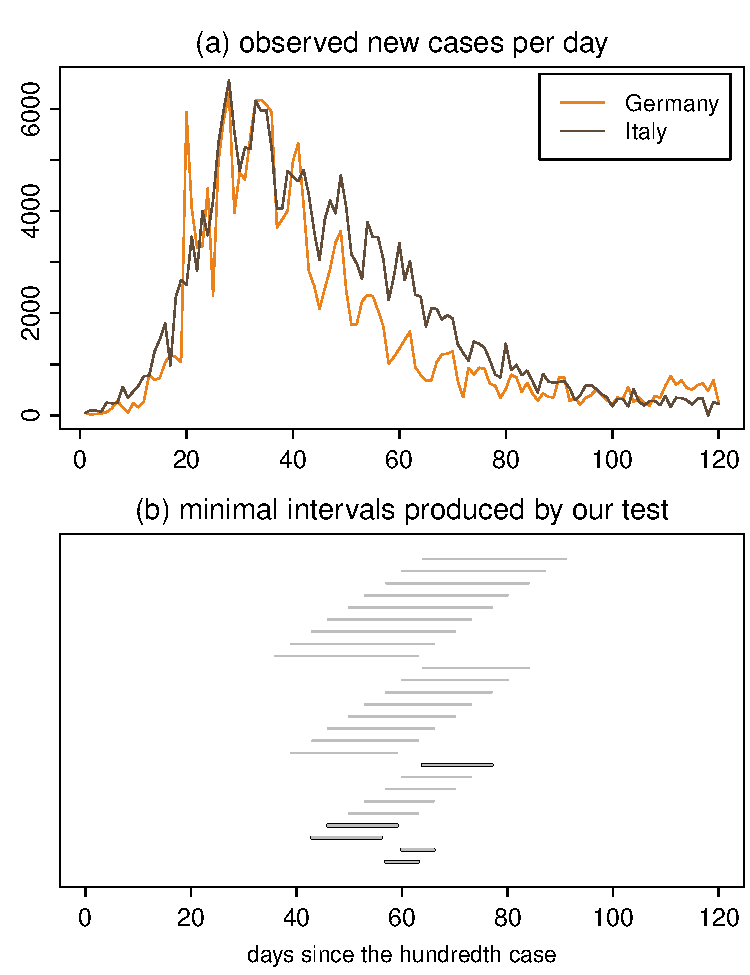
\includegraphics[width=0.49\textwidth]{plots/DEU_vs_ITA_presentation}
   		%\caption{Observed new cases per day in Germany and Italy}    			\label{fig:DEUvsITA}
		\hfill
		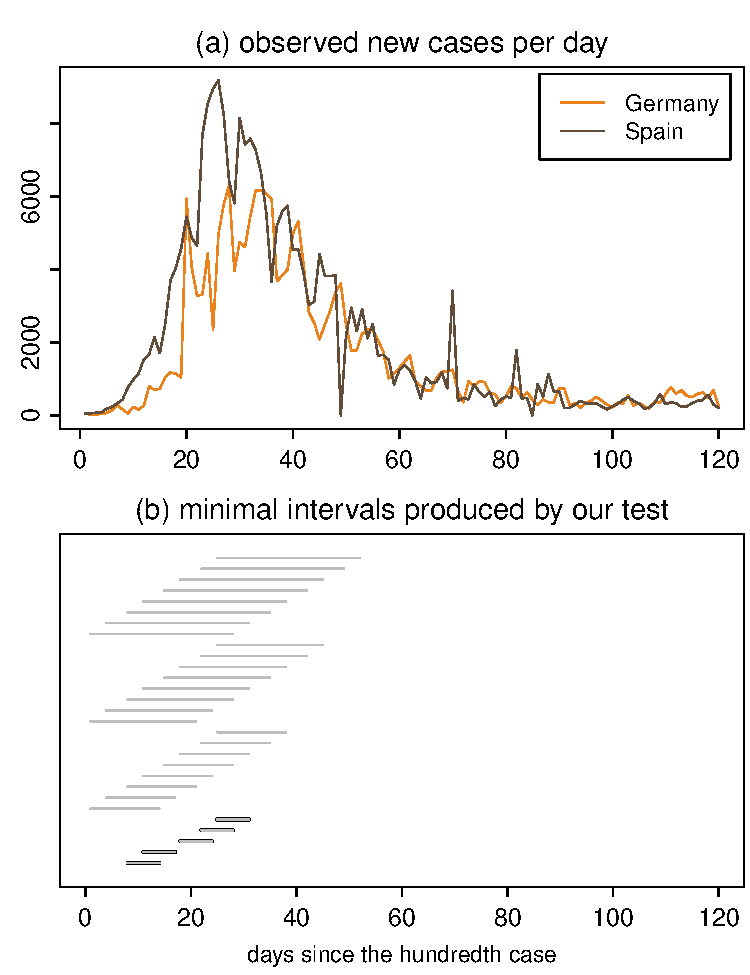
\includegraphics[width=0.49\textwidth]{plots/DEU_vs_ESP_presentation}
	\end{figure}
\end{frame}

\begin{frame}{Application results, part 2}
	\begin{figure}
		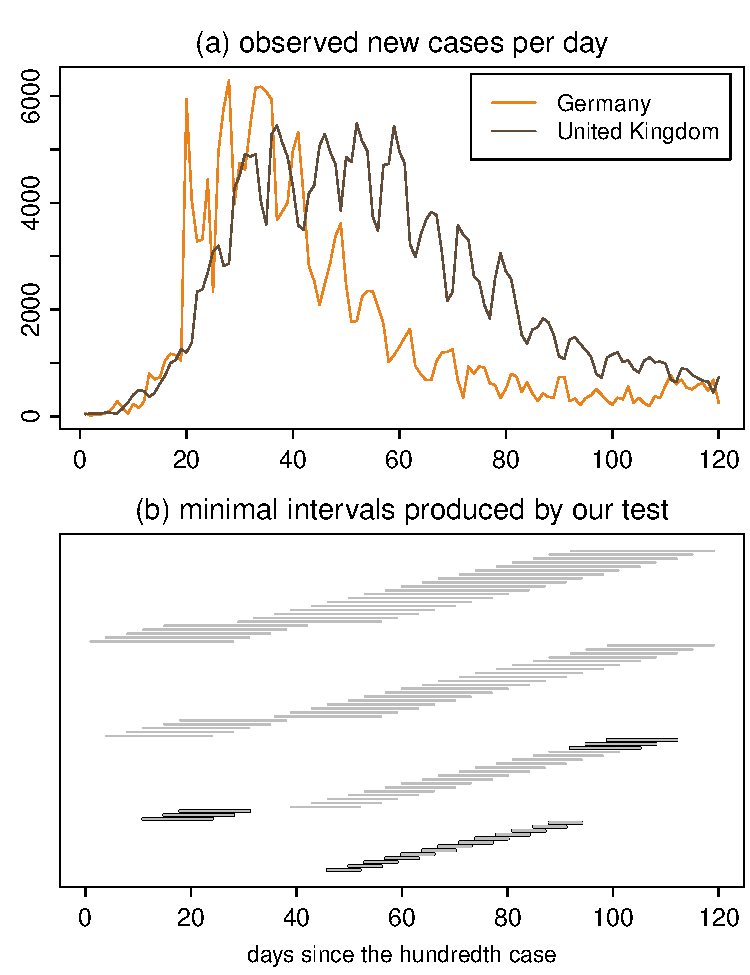
\includegraphics[width=0.49\textwidth]{plots/DEU_vs_GBR_presentation}
   		%\caption{Observed new cases per day in Germany and Italy}    			\label{fig:DEUvsITA}
		\hfill
		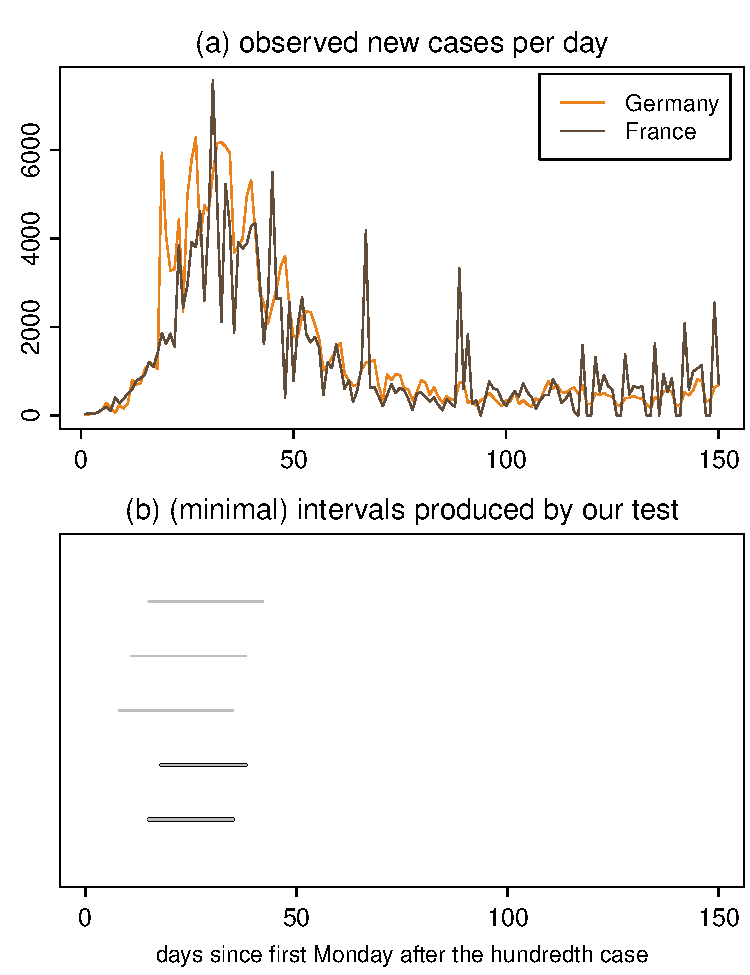
\includegraphics[width=0.49\textwidth]{plots/DEU_vs_FRA_presentation}
	\end{figure}
\end{frame}


\begin{frame}{Discussion}
We can claim, with confidence of about $95\%$, that the null hypothesis is violated for all intervals (and all pairs of countries) for which our test rejects the null. \pause

However, we can not say anything about the causes of such differences. This question requires further (probably not purely statistical) analysis.\pause

Further possible extensions:
\vspace{-1mm}
\begin{itemize}
	\item introduce scaling factor in the trend function, that allow for adjusting for the size of the country (population, density, testing regimes, etc.);\pause
	\item connect with data-driven techniques such as machine learning;\pause
	\item cluster the countries based on the trends they exhibit.
\end{itemize}
\end{frame}

\begin{frame}[standout]
  Thank you!
\end{frame}


\appendix

\begin{frame}{Simulation results for the size of the test}
\begin{figure}[t!]
	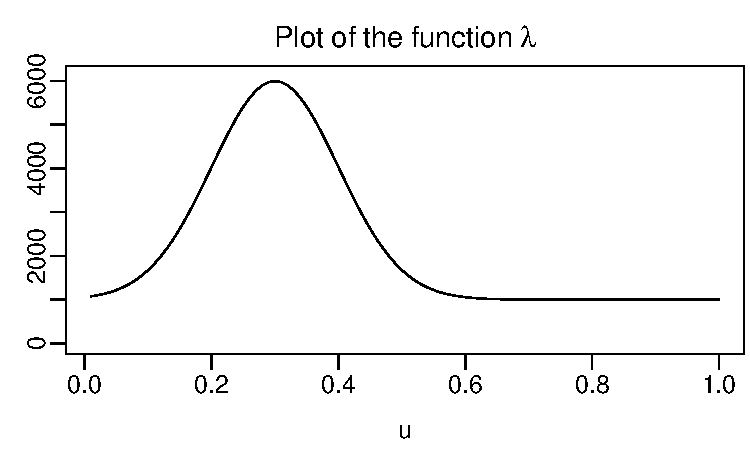
\includegraphics[height = 0.4\textheight]{plots/lambda_fct}
\end{figure}
\vspace{-2mm}
\scriptsize{\begin{table}[t]
\begin{center}
\caption{Size of the multiscale test}
\label{tab:size_shape}
% latex table generated in R 4.0.0 by xtable 1.8-4 package
% 
\begin{tabular}{ccccccccccccc}
  \hline
  \hline
100 &  & 0.010 & 0.035 & 0.070 &  & 0.008 & 0.030 & 0.058 &  & 0.004 & 0.024 & 0.052 \\ 
  250 &  & 0.007 & 0.030 & 0.072 &  & 0.007 & 0.037 & 0.072 &  & 0.006 & 0.034 & 0.064 \\ 
  500 &  & 0.005 & 0.029 & 0.064 &  & 0.003 & 0.021 & 0.049 &  & 0.004 & 0.028 & 0.058 \\ 
   \hline
\end{tabular}

\end{center}
\end{table}}
\end{frame}

\begin{frame}{Simulation results for the power of the test}
\begin{figure}[t!]
	\onslide<1->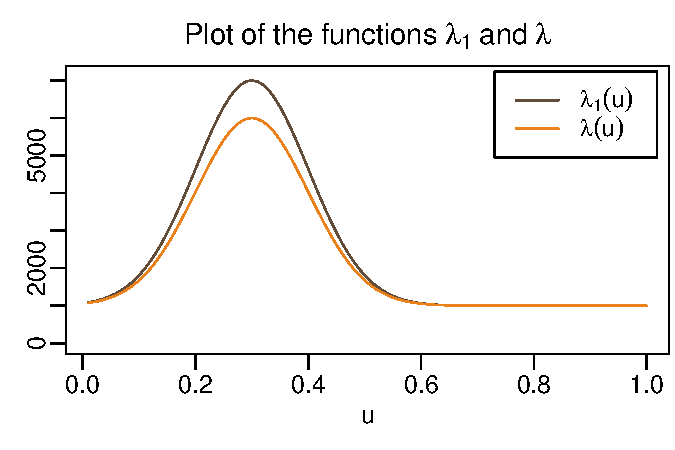
\includegraphics[width = 0.49\textwidth, height = 0.4\textheight]{plots/lambda_fcts_height}
	\onslide<2->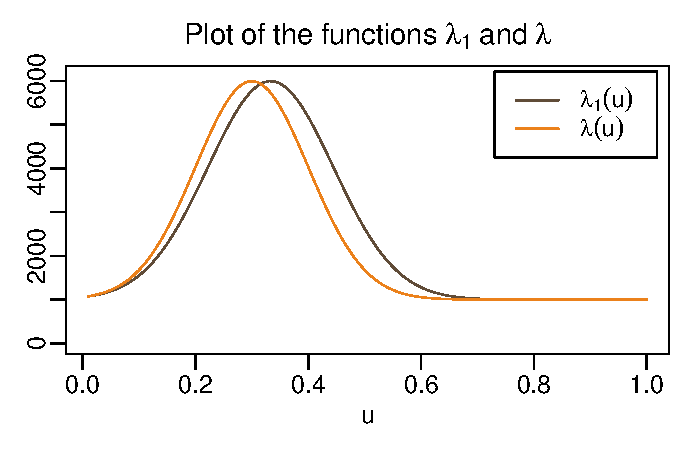
\includegraphics[width = 0.49\textwidth, height = 0.4\textheight]{plots/lambda_fcts_shift}	
\end{figure}\pause
\vspace{-5mm}
{\onslide<1>\scriptsize{\begin{table}[t]
\begin{center}
\caption{Power of the multiscale test for scenario A}
\label{tab:size_shape}
% latex table generated in R 3.6.1 by xtable 1.8-4 package
% 
\begin{tabular}{cccccccccc}
  \hline
  \hline
$T = 100$ & 0.335 & 0.518 & 0.597 & 0.306 & 0.474 & 0.545 & 0.212 & 0.352 & 0.418 \\ 
  $T = 250$ & 0.615 & 0.790 & 0.836 & 0.580 & 0.764 & 0.800 & 0.470 & 0.648 & 0.705 \\ 
  $T = 500$ & 0.736 & 0.905 & 0.917 & 0.738 & 0.884 & 0.890 & 0.636 & 0.799 & 0.830 \\ 
   \hline
\end{tabular}

\end{center}
\end{table}}}
{\onslide<2>
\vspace{-39.5mm}
\scriptsize{\begin{table}[t]
\begin{center}
\caption{Power of the multiscale test for scenario B}
\label{tab:size_shape}
% latex table generated in R 3.6.1 by xtable 1.8-4 package
% 
\begin{tabular}{cccccccccc}
  \toprule
 & \multicolumn{3}{c}{$n = 5$} & \multicolumn{3}{c}{$n = 10$} & \multicolumn{3}{c}{$n = 50$} \\
\cmidrule[0.4pt]{2-4} \cmidrule[0.4pt]{5-7} \cmidrule[0.4pt]{8-10}
 & \multicolumn{3}{c}{significance level $\alpha$} &\multicolumn{3}{c}{significance level $\alpha$} & \multicolumn{3}{c}{significance level $\alpha$} \\
 & 0.01 & 0.05 & 0.1  &  0.01 & 0.05 & 0.1  &  0.01 & 0.05 & 0.1 \\
\cmidrule[0.4pt]{1-10}
$T = 100$ & 0.824 & 0.910 & 0.903 & 0.812 & 0.893 & 0.890 & 0.738 & 0.847 & 0.857 \\ 
  $T = 250$ & 0.991 & 0.972 & 0.941 & 0.991 & 0.960 & 0.920 & 0.991 & 0.965 & 0.933 \\ 
  $T = 500$ & 0.997 & 0.973 & 0.949 & 0.995 & 0.961 & 0.923 & 0.996 & 0.969 & 0.932 \\ 
   \hline
\end{tabular}

\end{center}
\end{table}}}
\end{frame}

\begin{frame}[label = frame_sigma]{Estimator of ${\sigma}^2$}
We estimate the overdispersion paramter $\sigma^2$ by \[\widehat{\sigma}^2= \frac{1}{n} \sum_{i = 1}^n \hat{\sigma}_i^2 \text{ and } \hat{\sigma}_i^2 = \frac{\sum_{t=2}^T (X_{it}-X_{it-1})^2}{2 \sum_{t=1}^T X_{it}}\] \pause
We assume that $\lambda_i$ is Lipschitz continuous. Then
\[ X_{it} - X_{it-1} = \sigma \sqrt{\lambda_i\Big(\frac{t}{T}\Big)} (\eta_{it} - \eta_{it-1}) + r_{it}, \]
where $|r_{it}| \le C(1+|\eta_{it-1}|)/T$ with a sufficiently large $C$.\pause \, Hence,
\[ \frac{1}{T} \sum_{t=2}^T (X_{it} - X_{it-1})^2 = 2 \sigma^2 \Big\{ \frac{1}{T} \sum_{t=2}^T \lambda_i(t/T) \Big\} + o_p(1)\] \pause
Together with \[ \frac{1}{T} \sum_{t=1}^T X_{it} = \frac{1}{T} \sum_{t=1}^T \lambda_i(t/T) + o_p(1), \] we get that $\hat{\sigma}_i^2 = \sigma^2 + o_p(1)$ for any $i$ and thus $\hat{\sigma}^2 = \sigma^2 + o_p(1)$. \hyperlink{frame_teststatistic<4>}{\beamerbutton{Go back}}
\end{frame}


\begin{frame}[label = frame_notation]{Notation}
\begin{center}
In order to proceed with the proof, we will need the following notation:
\end{center}
\vspace{-2mm}
\begin{align*}
\widehat{\psi}_{ijk, T} &= \frac{\sum\nolimits_{t=1}^T \indsmall (X_{it} -X_{jt})}{\hat{\sigma} \big\{ \sum\nolimits_{t=1}^T \indsmall  (X_{it} + X_{jt} )\big\}^{1/2}} &&\\
\hat{\psi}_{ijk,T}^0 &= \frac{\sum\nolimits_{t=1}^T \indsmall \, \sigma \overline{\lambda}_{ij}^{1/2}(\frac{t}{T}) (\eta_{it} - \eta_{jt})}{ \hat{\sigma} \{ \sum\nolimits_{t=1}^T \indsmall (X_{it} + X_{jt}) \}^{1/2}} &&\hat{\Psi}_T^0 = \max_{(i,j,k)} a_k (|\hat{\psi}_{ijk,T}^0| - b_k)\\
\psi_{ijk,T}^0 &= \frac{1}{\sqrt{2Th_k}} \sum\limits_{t=1}^T \ind (\eta_{it} - \eta_{jt}) &&\Psi_T = \max_{(i,j,k)} a_k (|\psi_{ijk,T}^0| - b_k)\\
\phi_{ijk,T} &= \frac{1}{\sqrt{2 T h_k}} \sum\limits_{t=1}^T \ind (Z_{it} - Z_{jt}) &&\Phi_T = \max_{(i,j,k)} a_k (|\phi_{ijk,T}| - b_k)
\end{align*}
\end{frame}

\begin{frame}{Strategy of the proof}
\begin{enumerate}
\item We prove that  $\big| \hat{\Psi}_T^0 - \Psi_T \big| = o_p(r_T)$, where $\{r_T\}$ is some null sequence.\pause
\item With the help of results from Chernozhukov et al. (2017), we prove
\begin{equation*}\label{eq:kolmogorov-distance}
\sup_{q \in \mathbf{R}} \Big| \Prob\big( \Psi_T \le q \big) - \Prob\big( \Phi_T \le q \big) \Big| = o(1)
\end{equation*}\pause
\vspace{-2mm}
\item By using these two results, we now show that 
\begin{equation}\label{eq:kolmogorov-distance-hat}
\sup_{q \in \mathbb{R}} \Big| \Prob\big( \hat{\Psi}_T^0 \le q \big) - \Prob\big( \Phi_T \le q \big) \Big| = o(1)
\end{equation}\pause
\vspace{-2mm}
\item It can be shown that $\Prob (\Phi_T \le q_{T,\text{Gauss}}(\alpha)) = 1-\alpha$. From this and \eqref{eq:kolmogorov-distance-hat}, it immediately follows that  
\begin{equation*}
\Prob\big( \hat{\Psi}_T^0 \le q_{T,\text{Gauss}}(\alpha) \big) = 1 - \alpha + o(1), 
\end{equation*}
which in turn implies the desired statement. 
\end{enumerate}
\end{frame}



\begin{frame}{Idea behind the additive correction}
Consider the uncorrected Gaussian statistic
\begin{align*}
\Phi_{T}^{\text{uncor}} = \max_{(i,j,k)} |\phi_{ijk, T}|
\end{align*}\pause
and let the family of intervals be \[\mathcal{F} = \big\{[(m-1) h_l, m h_l] \text{ for } 1\le m \le 1/h_l, 1 \le l \le L\big\}\]\pause
Then we can rewrite the uncorrected test statistic as
\begin{align*}
\Phi_{T}^{\text{uncor}} = \max_{i, j} \max_{\substack{1 \le l \le L, \\ 1\le m \le 1/h_l}} \Big|\frac{1}{\sqrt{2 T h_l}} \sum\limits_{t=1}^T 1 \Big( \frac{t}{T} \in [(m-1) h_l, m h_l] \Big) (Z_{it} - Z_{jt})\Big|
\end{align*}\pause
$\Rightarrow \quad \max_m \ldots =\sqrt{2\log(1/h_l)} + o_P(1) \to \infty$ as $h \to 0$ and the stochastic behavior of $\Phi_{T}^{\text{uncor}}$ is dominated by the elements with small bandwidths $h_l$. \hyperlink{frame_test<4>}{\beamerbutton{Go back}}
\end{frame}



\end{document}
